\documentclass[aspectratio=169]{beamer}

\usetheme{Boadilla}
\useinnertheme{rounded}
\usefonttheme{professionalfonts}
\setbeamertemplate{navigation symbols}{}

\usepackage[T1]{fontenc}
\usepackage[utf8]{inputenc}
\usepackage{lmodern}
\usepackage{booktabs}
\usepackage{array}
\usepackage{colortbl}
\usepackage{tabularx}
\usepackage{tikz}
\usetikzlibrary{positioning,arrows.meta,shapes.geometric}

\definecolor{TitleBlue}{RGB}{18,47,92}
\definecolor{AccentTeal}{RGB}{30,114,120}
\definecolor{AccentGold}{RGB}{201,146,42}
\definecolor{CriticalRed}{RGB}{167,43,43}
\definecolor{SoftGray}{RGB}{82,82,82}
\definecolor{LightBlue}{RGB}{232,240,250}
\definecolor{PanelGray}{RGB}{245,247,250}
\definecolor{WhiteText}{RGB}{250,250,250}
\definecolor{RowTintA}{RGB}{247,249,252}
\definecolor{RowTintB}{RGB}{236,244,248}
\definecolor{GreenOk}{RGB}{30,120,60}
\definecolor{LightGreen}{RGB}{220,245,228}

\setbeamercolor{background canvas}{bg=white}
\setbeamercolor{title}{fg=white}
\setbeamercolor{subtitle}{fg=white}
\setbeamercolor{author}{fg=white}
\setbeamercolor{institute}{fg=white}
\setbeamercolor{date}{fg=white}
\setbeamercolor{frametitle}{fg=white,bg=TitleBlue}
\setbeamercolor{structure}{fg=TitleBlue}
\setbeamercolor{normal text}{fg=black}
\setbeamercolor{section in toc}{fg=TitleBlue}
\setbeamercolor{block title}{fg=white,bg=AccentTeal}
\setbeamercolor{block body}{bg=LightBlue}
\setbeamercolor{alertblock title}{fg=white,bg=CriticalRed}
\setbeamercolor{alertblock body}{bg=CriticalRed!10}
\setbeamercolor{exampleblock title}{fg=white,bg=GreenOk}
\setbeamercolor{exampleblock body}{bg=LightGreen}
\setbeamercolor{item projected}{bg=AccentGold,fg=white}
\setbeamercolor{footline}{fg=white,bg=TitleBlue}

\setbeamerfont{title}{series=\bfseries,size=\LARGE}
\setbeamerfont{subtitle}{size=\large}
\setbeamerfont{frametitle}{series=\bfseries,size=\large}
\setbeamerfont{section title}{series=\bfseries,size=\Large}

\setbeamertemplate{blocks}[rounded][shadow=false]

\tikzset{
  pipebox/.style={
    rectangle, rounded corners=3pt, draw=TitleBlue, fill=LightBlue, thick,
    align=center, minimum width=2.45cm, minimum height=0.95cm, font=\footnotesize
  },
  pipeboxA/.style={
    rectangle, rounded corners=4pt, draw=TitleBlue, fill=LightBlue, thick,
    align=center, text width=3.4cm, minimum height=0.95cm, font=\footnotesize
  },
  pipeboxB/.style={
    rectangle, rounded corners=4pt, draw=AccentTeal, fill=PanelGray, thick,
    align=center, text width=3.4cm, minimum height=0.95cm, font=\footnotesize
  },
  pipeboxC/.style={
    rectangle, rounded corners=4pt, draw=AccentGold!80!black, fill=AccentGold!14, thick,
    align=center, text width=3.4cm, minimum height=0.95cm, font=\footnotesize
  },
  pipeboxS/.style={
    rectangle, rounded corners=3pt, draw=TitleBlue, fill=LightBlue, thick,
    align=center, minimum width=1.8cm, minimum height=0.85cm, font=\scriptsize
  },
  pipeboxS2/.style={
    rectangle, rounded corners=3pt, draw=AccentTeal, fill=PanelGray, thick,
    align=center, minimum width=1.8cm, minimum height=0.85cm, font=\scriptsize
  },
  pipeboxSG/.style={
    rectangle, rounded corners=3pt, draw=GreenOk, fill=LightGreen, thick,
    align=center, minimum width=1.8cm, minimum height=0.85cm, font=\scriptsize
  },
  criticalbox/.style={
    rectangle, rounded corners=4pt, draw=CriticalRed, fill=CriticalRed!10, thick,
    align=center, text width=3.6cm, minimum height=0.9cm
  },
  pipebox2/.style={
    rectangle, rounded corners=3pt, draw=AccentTeal, fill=PanelGray, thick,
    align=center, minimum width=2.45cm, minimum height=0.95cm
  },
  pipearrow/.style={
    -{Latex[length=2.5mm,width=1.8mm]}, thick, draw=TitleBlue
  },
  pipearrowG/.style={
    -{Latex[length=2.5mm,width=1.8mm]}, thick, draw=AccentTeal
  }
}

\setbeamertemplate{frametitle}{
  \vspace{0.15em}
  \begin{beamercolorbox}[wd=\paperwidth,ht=3.2ex,dp=1.2ex,leftskip=0.8cm,rightskip=0.3cm]{frametitle}
    \insertframetitle
  \end{beamercolorbox}
}

\setbeamertemplate{footline}{
  \leavevmode
  \hbox{
    \begin{beamercolorbox}[wd=.28\paperwidth,ht=2.8ex,dp=1.1ex,leftskip=.4cm]{footline}
      \scriptsize \insertshortauthor
    \end{beamercolorbox}
    \begin{beamercolorbox}[wd=.54\paperwidth,ht=2.8ex,dp=1.1ex,center]{footline}
      \scriptsize \insertsectionhead
    \end{beamercolorbox}
    \begin{beamercolorbox}[wd=.18\paperwidth,ht=2.8ex,dp=1.1ex,rightskip=.4cm]{footline}
      \hfill \scriptsize \insertframenumber/\inserttotalframenumber
    \end{beamercolorbox}
  }
}

\setbeamertemplate{title page}{
  \begin{tikzpicture}[remember picture,overlay]
    \fill[TitleBlue] (current page.south west) rectangle (current page.north east);
    \fill[AccentTeal] (current page.south west) rectangle ([xshift=3.2cm,yshift=1.1cm]current page.south west);
    \fill[AccentGold] ([xshift=-3.0cm]current page.north east) rectangle (current page.north east);
  \end{tikzpicture}
  \vspace{1.3cm}
  \begin{flushleft}
    {\usebeamerfont{title}\usebeamercolor[fg]{title}\inserttitle\par}
    \vspace{0.4cm}
    {\usebeamerfont{subtitle}\usebeamercolor[fg]{subtitle}\insertsubtitle\par}
    \vspace{1.2cm}
    {\large \insertauthor\par}
    \vspace{0.2cm}
    {\normalsize \insertinstitute\par}
    \vspace{0.2cm}
    {\normalsize \insertdate\par}
  \end{flushleft}
  \vfill
}

\title{Charting Student Math Misunderstandings}
\subtitle{Qwen3-8B, Explainable AI, and Ontology-Aware Pipeline}
\author[ML Project Team]{Age of Ultron}
\institute{CSE 330 --- Machine Learning Sessional}
\date{}

% ============================================================
\begin{document}
% ============================================================

% ------ TITLE -----------------------------------------------
\section{Title}
\begin{frame}
  \titlepage
\end{frame}

% ------ ROADMAP ---------------------------------------------
\section{Roadmap}
\begin{frame}{Presentation Roadmap}
\small
\begin{columns}[T]
\column{0.48\textwidth}
\begin{enumerate}
  \item \textbf{Problem Statement}\\{\scriptsize What are we solving and why?}
  \vspace{4pt}
  \item \textbf{Dataset \& Benchmark}\\{\scriptsize MAP Kaggle competition data}
  \vspace{4pt}
  \item \textbf{Model Evolution Journey}\\{\scriptsize DeBERTa $\rightarrow$ Qwen3-8B, step by step}
  \vspace{4pt}
  \item \textbf{Training: QLoRA + Regularization}\\{\scriptsize AWP, R-Drop, EMA, Layerwise LR}
\end{enumerate}
\column{0.48\textwidth}
\begin{enumerate}
  \setcounter{enumi}{4}
  \item \textbf{Full Pipeline (rf.ipynb)}\\{\scriptsize KB, Graph, GraphRAG, Counterfactual, Ensemble}
  \vspace{4pt}
  \item \textbf{Inference \& Explainable AI}\\{\scriptsize rf\_inf\_expAi: Phase 1 + Phase 2}
  \vspace{4pt}
  \item \textbf{Score Progression \& Results}\\{\scriptsize MAP@3: 0.65 $\rightarrow$ 0.80 $\rightarrow$ 0.93999}
  \vspace{4pt}
  \item \textbf{Research Papers \& Conclusion}\\{\scriptsize 20+ referenced works}
\end{enumerate}
\end{columns}
\end{frame}

% ============================================================
\section{Problem \& Data}
% ============================================================

% ------ PROBLEM STATEMENT -----------------------------------
\begin{frame}{Problem Statement}
\begin{columns}[T]
\column{0.55\textwidth}
\begin{itemize}
  \item \textbf{The Challenge:} Identifying an incorrect answer is straightforward, but understanding the underlying \textit{misconception} causing the systematic error is hard.
  \item \textbf{Objective:} Build an ML pipeline to automatically classify the specific mathematical misconception based on:
  \begin{itemize}
    \item The question text
    \item The student's chosen (incorrect) answer
    \item The student's written reasoning
  \end{itemize}
  \item \textbf{Explainability Requirement:} Incorporate XAI to provide transparent, interpretable rationales.
  \item \textbf{Educational Impact:} Allow teachers to understand cognitive gaps and design targeted interventions.
\end{itemize}
\column{0.42\textwidth}
\begin{block}{Evaluation Metric: MAP@3}
Mean Average Precision at rank 3.\\[4pt]
For each test row, predict the correct misconception within your top-3 ranked candidates:
\[
  \text{MAP@3} = \frac{1}{\text{rank}} \;\text{ if found in top-3}
\]
\begin{center}
\begin{tabular}{cc}
\toprule
\textbf{Correct at Rank} & \textbf{Score}\\
\midrule
1 & 1.000\\
2 & 0.500\\
3 & 0.333\\
Not found & 0.000\\
\bottomrule
\end{tabular}
\end{center}
MAP@3 = average over all rows.
\end{block}
\end{columns}
\end{frame}

% ------ DATASET OVERVIEW ------------------------------------
\begin{frame}{Dataset: MAP --- Charting Student Math Misunderstandings}
\begin{columns}[T]
\column{0.54\textwidth}
\begin{itemize}
  \item \textbf{Source:} Kaggle --- Eedi \& Vanderbilt University
  \item \textbf{Question Data:} Subject, mathematical construct (skill), full question text
  \item \textbf{Student Responses:} Chosen multiple-choice answer + written explanation
  \item \textbf{Correctness Flag:} Boolean --- is the selected answer valid?
  \item \textbf{Target Labels (Train Only):}
  \begin{itemize}
    \item \textbf{Category:} Relationship type (e.g., \texttt{True\_Misconception}, \texttt{False\_Correct})
    \item \textbf{Misconception:} Specific math misconception label (or \texttt{NA} if none)
  \end{itemize}
\end{itemize}
\column{0.43\textwidth}
\begin{block}{Dataset Statistics}
\begin{tabular}{ll}
Training rows & 36{,}696 \\
Target labels (Category) & 65 \\
Unique misconceptions & 2{,}587 \\
Training question IDs & 15 \\
% Test question IDs & 5 \\
\end{tabular}
\end{block}
\vspace{6pt}
\begin{alertblock}{Key Challenge}
\textbf{Highly imbalanced:}\\
\texttt{True\_Correct:NA} dominates.\\
Each question supports only 6--11 valid labels.\\
The effective label space is very small per instance.
\end{alertblock}
\end{columns}
\end{frame}

% ------ DATASET STATS ---------------------------------------
\begin{frame}{Dataset: Label Structure}
\begin{itemize}
  \item Training data contains 36,696 rows, 65 target labels, and 15 training question IDs.
  \item The label distribution is highly imbalanced; \texttt{True\_Correct:NA} is the dominant class.
  \item Each question supports only a small subset of labels, typically around 6--11.
  \item After conditioning on whether the selected answer is correct, the effective label space becomes even smaller.
  \item This is a relatively \textbf{closed-world benchmark}: test examples stay close to the same question and label universe seen during training.
  \item The competition requires predicting the exact misconception string from 2,587 possible classes --- a very fine-grained multi-class problem.
\end{itemize}
\end{frame}

% ------ DATASET EXAMPLE -------------------------------------
\begin{frame}{Dataset Example (Sample Rows)}
\scriptsize
\setlength{\tabcolsep}{3pt}
\renewcommand{\arraystretch}{1.15}
\begin{table}
\centering
\resizebox{\textwidth}{!}{%
\begin{tabular}{|p{4.0cm}|p{1.5cm}|p{6.2cm}|p{2.4cm}|p{2.6cm}|}
\hline
\textbf{QuestionText} & \textbf{MC\_Answer} & \textbf{StudentExplanation} & \textbf{Category} & \textbf{Misconception} \\ \hline
If $2y = 24$, what is the value of $y$? &
$48$ &
You need to do $24 \times 2$ to get the answer of $y$, which is $48$. &
False\_Misconception &
Inverse\_operation \\ \hline
Calculate $\frac{2}{3}\times 5$ &
$3\frac{1}{3}$ &
Because $2\times 5=10$ and $3\times 3=9$, so there will be three wholes and 1 left over. &
True\_Correct &
NA \\ \hline
Calculate $\frac{2}{3}\times 5$ &
$3\frac{1}{3}$ &
See also $2.5$, finding the correct score is $3\frac{1}{3}$. &
True\_Neither &
NA \\ \hline
\end{tabular}%
}
\caption{Example records showing question text, selected answer, explanation, category, and misconception label.}
\end{table}
\vspace{-4pt}
\begin{exampleblock}{Key Insight}
The same question-answer pair can have \textit{different} misconceptions depending on the student's written explanation. The explanation text is the most informative feature.
\end{exampleblock}
\end{frame}

% ============================================================
\section{Model Evolution}
% ============================================================

% ------ EVOLUTION OVERVIEW ----------------------------------
\begin{frame}{The Journey: From 0.65 to 0.93999}
\small
\setlength{\tabcolsep}{4pt}
\renewcommand{\arraystretch}{1.3}
\begin{center}
\begin{tabular}{clp{5.2cm}c}
\toprule
\textbf{\#} & \textbf{Notebook} & \textbf{Key Innovation} & \textbf{MAP@3}\\
\midrule
\rowcolor{RowTintA}
1 & DeBERTa baseline & Fine-tune encoder (435M params), GroupKFold, EMA & 0.65\\
\rowcolor{RowTintB}
2 & DeBERTa + Suffix & Semantic label format, multi-seed ensemble & 0.80\\
\rowcolor{RowTintA}
3 & Qwen3-8B training & QLoRA + AWP + R-Drop + EMA + Label Smooth & \textit{training}\\
\rowcolor{RowTintB}
4 & Qwen3-8B simple infer & Load adapter, classify, submit & 0.93999\\
\rowcolor{LightBlue}
5 & rf.ipynb & KB + Graph + GraphRAG + Counterfactual + Ensemble & \textit{pipeline}\\
\rowcolor{LightGreen}
6 & \textbf{rf\_inf\_expAi} & \textbf{Phase 1 classify + Phase 2 Explainable AI} & \textbf{0.93999}\\
\bottomrule
\end{tabular}
\end{center}
\vspace{6pt}
\begin{center}
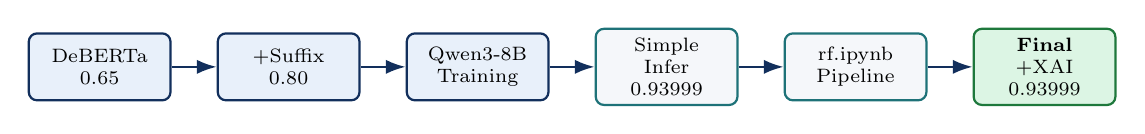
\begin{tikzpicture}
  \node[pipeboxS]  (s1) at (0,0)      {DeBERTa\\0.65};
  \node[pipeboxS]  (s2) at (2.4,0)    {+Suffix\\0.80};
  \node[pipeboxS]  (s3) at (4.8,0)    {Qwen3-8B\\Training};
  \node[pipeboxS2] (s4) at (7.2,0)    {Simple\\Infer\\0.93999};
  \node[pipeboxS2] (s5) at (9.6,0)    {rf.ipynb\\Pipeline};
  \node[pipeboxSG] (s6) at (12.0,0)   {\textbf{Final}\\+XAI\\0.93999};
  \draw[pipearrow] (s1)--(s2); \draw[pipearrow] (s2)--(s3);
  \draw[pipearrow] (s3)--(s4); \draw[pipearrow] (s4)--(s5);
  \draw[pipearrow] (s5)--(s6);
\end{tikzpicture}
\end{center}
\end{frame}

% ------ STAGE 1: DeBERTa ------------------------------------
\begin{frame}{Stage 1: DeBERTa-v3-Large Baseline \texorpdfstring{--- MAP@3 = 0.65}{}}
\begin{columns}[T]
\column{0.52\textwidth}
\begin{block}{What We Did}
\begin{itemize}
  \item Fine-tuned \textbf{DeBERTa-v3-Large} (435M parameters) as a multi-class classifier over 65 misconception categories.
  \item \textbf{5-fold GroupKFold} cross-validation: groups by Question ID, so the same question never appears in both train and validation folds.
  \item \textbf{EMA} (Exponential Moving Average, decay = 0.999) over model weights for stable inference.
  \item Ensemble: average logits across all 5 folds, then \textbf{temperature scaling} to calibrate probabilities.
\end{itemize}
\end{block}
\column{0.45\textwidth}
\begin{alertblock}{Limitation Discovered}
\begin{itemize}
  \item Labels were raw integer IDs (e.g., 47, 1203, 2041).
  \item The 2587-class output head was essentially a random lookup table --- no semantic structure.
  \item Top-1 accuracy $\approx$ 54\%: the model often ranked the correct answer 2nd or 3rd, not 1st.
  \item DeBERTa \textbf{pattern-matches}; it cannot reason about the meaning of a misconception.
\end{itemize}
\end{alertblock}
\vspace{6pt}
\begin{center}
{\Large\color{TitleBlue} MAP@3 = \textbf{0.65}}
\end{center}
\end{columns}
\end{frame}

% ------ STAGE 2: SUFFIX CLASSIFICATION ----------------------
\begin{frame}{Stage 2: Suffix Classification --- MAP@3 = 0.80 \texorpdfstring{(+0.15)}{}}
\begin{columns}[T]
\column{0.50\textwidth}
\begin{block}{Key Innovation: Label Representation}
Instead of predicting integer IDs, the target string became:
\begin{center}
\texttt{``Category:MisconceptionText''}\\[4pt]
e.g., \texttt{``Fractions:Divides numerator}\\
\texttt{and denominator separately''}
\end{center}
This is \textbf{suffix classification}: the model sees \textit{what a misconception means} in the label itself, not just a number.
\end{block}
\vspace{6pt}
\begin{block}{Additional Improvements}
\begin{itemize}
  \item \textbf{Multi-seed $\times$ 5 folds}: more diverse checkpoints, lower variance ensemble.
  \item \textbf{Temperature search on MAP@3} (not cross-entropy) --- task-aligned calibration.
  \item Added a \textbf{knowledge base} with Qwen2.5-7B-Instruct explanations per misconception.
\end{itemize}
\end{block}
\column{0.47\textwidth}
\begin{exampleblock}{Why This Worked So Well}
DeBERTa's attention mechanism can now exploit \textbf{words in the label}:
\begin{itemize}
  \item ``Fractions'' and ``Divides'' are meaningful tokens.
  \item Similar misconceptions share similar vocabulary $\Rightarrow$ the model clusters them correctly.
  \item The +0.15 MAP@3 gain came almost entirely from this one change.
\end{itemize}
\end{exampleblock}
\vspace{6pt}
\begin{alertblock}{Remaining Gap}
DeBERTa (435M) still pattern-matches. For \textit{ambiguous} student explanations --- where misconceptions share similar phrasing --- it confuses them. We need a model that can \textbf{reason}, not just match.
\end{alertblock}
\end{columns}
\end{frame}

% ============================================================
\section{Training Details}
% ============================================================

% ------ WHY QWEN3-8B ----------------------------------------
\begin{frame}{Stage 3: Why Switch to Qwen3-8B?}
\begin{columns}[T]
\column{0.48\textwidth}
\begin{block}{The Case for a Larger Model}
\begin{tabular}{lll}
\toprule
 & \textbf{DeBERTa} & \textbf{Qwen3-8B}\\
\midrule
Parameters & 435M & 8B ($\times$18)\\
Architecture & Encoder-only & Decoder (full)\\
Reasoning & Pattern match & Deep attention\\
Context & 512 tokens & 8192 tokens\\
Role & Discriminator & Understander\\
\bottomrule
\end{tabular}
\end{block}
\vspace{8pt}
\begin{itemize}
  \item Loaded as \texttt{AutoModelForSequenceClassification}: the full 32-layer Transformer processes the student explanation through all attention heads before the classification head.
  \item Much larger capacity $\Rightarrow$ can capture nuanced distinctions between similar misconceptions.
\end{itemize}
\column{0.48\textwidth}
\begin{alertblock}{The GPU Memory Problem}
An 8B parameter model in fp32 requires $\approx$32 GB VRAM.\\
Kaggle provides only \textbf{16 GB VRAM} (T4/P100).\\[6pt]
Full fine-tuning is \textbf{impossible} with available hardware.
\end{alertblock}
\vspace{8pt}
\begin{exampleblock}{Solution: QLoRA}
\textbf{Q}uantized \textbf{Lo}w-\textbf{R}ank \textbf{A}daptation:\\
\begin{enumerate}
  \item Freeze the base model in \textbf{4-bit NF4} quantization.
  \item Add small trainable rank-16 matrices (LoRA adapters) to attention layers.
  \item Train \textit{only} the adapters ($\approx$0.1\% of parameters).
  \item Adapter size: $\approx$200 MB vs.\ full model's 16 GB.
\end{enumerate}
\end{exampleblock}
\end{columns}
\end{frame}

% ------ QLoRA -----------------------------------------------
\begin{frame}{QLoRA: Parameter-Efficient Fine-Tuning}
\begin{columns}[T]
\column{0.48\textwidth}
\begin{block}{LoRA (Hu et al., 2022)}
For each attention weight matrix $W \in \mathbb{R}^{d\times k}$:
\[
  W' = W + \Delta W = W + BA
\]
where $B \in \mathbb{R}^{d\times r}$, $A \in \mathbb{R}^{r\times k}$, rank $r \ll \min(d,k)$.\\[6pt]
Only $B$ and $A$ are trained. $W$ stays frozen.
\end{block}
\vspace{6pt}
\begin{block}{QLoRA (Dettmers et al., 2023)}
Adds 4-bit NF4 quantization to the frozen base:
\begin{itemize}
  \item \texttt{BitsAndBytesConfig(load\_in\_4bit=True,}\\
        \texttt{\quad bnb\_4bit\_quant\_type="nf4",}\\
        \texttt{\quad bnb\_4bit\_compute\_dtype=bfloat16)}
  \item Dequantize only when computing forward pass.
  \item Entire 8B model fits in 10 GB VRAM during training.
\end{itemize}
\end{block}
\column{0.48\textwidth}
\begin{block}{Our LoRA Configuration}
\begin{tabular}{ll}
\toprule
Parameter & Value\\
\midrule
Rank $r$ & 16\\
$\alpha$ & 32\\
Dropout & 0.05\\
Target modules & All attention\\
Trainable params & $\approx$0.1\%\\
Adapter file size & $\approx$200 MB\\
\bottomrule
\end{tabular}
\end{block}
\vspace{8pt}
\begin{exampleblock}{Output Artifacts}
After training, two files are saved and used by all downstream notebooks:
\begin{itemize}
  \item \texttt{adapter\_model.safetensors}\\(LoRA weights)
  \item \texttt{label\_encoder.joblib}\\(misconception index $\leftrightarrow$ label string)
\end{itemize}
\end{exampleblock}
\end{columns}
\end{frame}

% ------ TRAINING REGULARIZATION -----------------------------
\begin{frame}{Training Regularization: AWP + R-Drop + EMA}
\begin{columns}[T]
\column{0.32\textwidth}
\begin{block}{AWP (Wu et al., 2020)}
\textbf{Adversarial Weight Perturbation}\\[4pt]
After normal backward pass, slightly perturb model weights:
\[
  w' = w + \varepsilon\,\frac{\nabla_w \mathcal{L}}{\|\nabla_w \mathcal{L}\|}
\]
Compute perturbed loss $\mathcal{L}'$, then restore $w$.\\[4pt]
Flattens the loss surface $\Rightarrow$ better generalization.\\[4pt]
\textbf{Config:} lr = 0.1, $\varepsilon$ = 1e-4, starts epoch 1.\\[4pt]
\textbf{Reported gain:} +1.0--2.0\% MAP
\end{block}
\column{0.32\textwidth}
\begin{block}{R-Drop (Liang et al., 2021)}
\textbf{Regularized Dropout}\\[4pt]
Two forward passes with dropout active, producing $p_1$ and $p_2$.
\[
  \mathcal{L} = \frac{\mathcal{L}_1 + \mathcal{L}_2}{2} + \alpha\, \text{KL}(p_1 \| p_2)
\]
Forces the model to give \textit{consistent} predictions across dropout masks.\\[4pt]
\textbf{Config:} $\alpha$ = 0.5\\[4pt]
\textbf{Reported gain:} +0.5--1.5\% MAP
\end{block}
\column{0.32\textwidth}
\begin{block}{EMA (Tarvainen \& Valpola, 2017)}
\textbf{Exponential Moving Average}\\[4pt]
Maintain a shadow copy of weights:
\[
  \theta_{\text{EMA}} \leftarrow m\,\theta_{\text{EMA}} + (1-m)\,\theta
\]
where $m = 0.999$. The EMA model is \textit{smoother} than the instantaneous checkpoint.\\[4pt]
Apply EMA weights at evaluation and final save.\\[4pt]
\textbf{Reported gain:} +0.3--0.8\% MAP
\end{block}
\end{columns}
\end{frame}

% ------ COMPLETE TRAINING RECIPE ----------------------------
\begin{frame}{Complete Training Recipe (Notebook 3)}
\begin{columns}[T]
\column{0.48\textwidth}
\begin{block}{Full Technique Stack}
\footnotesize
\setlength{\tabcolsep}{4pt}
\renewcommand{\arraystretch}{1.2}
\begin{tabular}{p{2.6cm}p{4.0cm}}
\toprule
\textbf{Technique} & \textbf{Config / Gain}\\
\midrule
QLoRA (4-bit NF4) & r=16, $\alpha$=32, fits 16 GB VRAM\\
R-Drop & $\alpha$=0.5, +0.5--1.5\% MAP\\
AWP & lr=0.1, $\varepsilon$=1e-4, +1.0--2.0\% MAP\\
EMA & decay=0.999, +0.3--0.8\% MAP\\
Label Smoothing & Prevents overconfidence (2587 classes)\\
Layerwise LR decay & 0.95$\times$ per layer (ULMFiT style)\\
AdamW optimizer & Decoupled weight decay\\
Gradient clipping & max\_norm = 1.0\\
StratifiedGroupKFold & No question leakage across folds\\
\bottomrule
\end{tabular}
\end{block}
\column{0.48\textwidth}
\begin{block}{Why Layerwise LR Decay?}
Lower Transformer layers hold \textbf{general} language representations built during pre-training on billions of tokens. Higher layers are more \textbf{task-specific}.\\[6pt]
Giving lower layers a smaller learning rate (decay = 0.95 per layer) preserves these representations and lets only the top layers adapt aggressively.\\[6pt]
Introduced by Howard \& Ruder (ULMFiT, 2018).
\end{block}
\vspace{8pt}
\begin{exampleblock}{Combined Effect}
All techniques stack: the final Qwen3-8B adapter trained with this recipe achieved \textbf{MAP@3 = 0.93999} on simple inference --- a 0.14 jump over the best DeBERTa ensemble.
\end{exampleblock}
\end{columns}
\end{frame}

% ------ STAGE 4: SIMPLE INFERENCE ---------------------------
\begin{frame}{Stage 4: Qwen3-8B Simple Inference --- 0.93999}
\begin{columns}[T]
\column{0.52\textwidth}
\begin{block}{What Notebook 4 Does}
\begin{enumerate}
  \item Load Qwen3-8B base model in 4-bit mode.
  \item Load LoRA adapter from \texttt{adapter\_model.safetensors}.
  \item Run forward pass on each test row through the 32-layer Transformer.
  \item Softmax over 2587-class head $\Rightarrow$ probability distribution.
  \item Decode top-12 indices via \texttt{label\_encoder.joblib}.
  \item Write \texttt{submission.csv} with top-12 candidates ranked by probability.
\end{enumerate}
\end{block}
\vspace{4pt}
\begin{center}
{\Large\color{GreenOk} Score: \textbf{0.93999}} \quad {\large $\uparrow$ from 0.80}
\end{center}
\column{0.44\textwidth}
\begin{alertblock}{Limitation: Black Box}
\begin{itemize}
  \item Single model, single stage.
  \item No external knowledge used.
  \item No re-ranking or error correction.
  \item If the model is wrong, there is nothing to catch it.
  \item Cannot explain \textit{why} a misconception was predicted.
\end{itemize}
\end{alertblock}
\vspace{8pt}
\begin{block}{What Comes Next}
The rf.ipynb and rf\_inf\_expAi notebooks build a full multi-stage pipeline \textit{around} this trained model to:
\begin{itemize}
  \item Add knowledge-guided re-ranking
  \item Add causal verification
  \item Add natural-language explanations
\end{itemize}
\end{block}
\end{columns}
\end{frame}

% ============================================================
\section{Full Pipeline}
% ============================================================

% ------ RF.IPYNB OVERVIEW -----------------------------------
\begin{frame}{rf.ipynb: Full 5-Stage Pipeline Overview}
\begin{center}
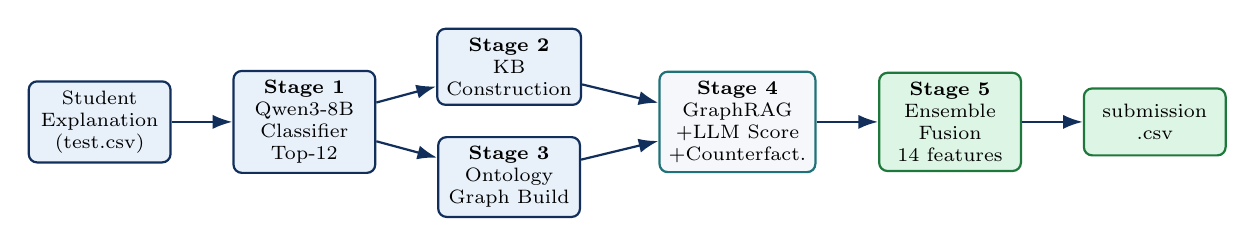
\begin{tikzpicture}
  \node[pipeboxS]  (inp) at (-1.6, 0)   {Student\\Explanation\\(test.csv)};
  \node[pipeboxS]  (s1)  at (1.0, 0)    {\textbf{Stage 1}\\Qwen3-8B\\Classifier\\Top-12};
  \node[pipeboxS]  (s2)  at (3.6, 0.7)  {\textbf{Stage 2}\\KB\\Construction};
  \node[pipeboxS]  (s3)  at (3.6,-0.7)  {\textbf{Stage 3}\\Ontology\\Graph Build};
  \node[pipeboxS2] (s4)  at (6.5, 0)    {\textbf{Stage 4}\\GraphRAG\\+LLM Score\\+Counterfact.};
  \node[pipeboxSG] (s5)  at (9.2, 0)    {\textbf{Stage 5}\\Ensemble\\Fusion\\14 features};
  \node[pipeboxSG] (out) at (11.8, 0)   {submission\\.csv};
  %
  \draw[pipearrow]  (inp) -- (s1);
  \draw[pipearrow]  (s1)  -- (s2);
  \draw[pipearrow]  (s1)  -- (s3);
  \draw[pipearrow]  (s2)  -- (s4);
  \draw[pipearrow]  (s3)  -- (s4);
  \draw[pipearrow]  (s4)  -- (s5);
  \draw[pipearrow]  (s5)  -- (out);
\end{tikzpicture}
\end{center}
\vspace{6pt}
\begin{columns}[T]
\column{0.48\textwidth}
\begin{block}{Cells in rf.ipynb}
\footnotesize
\begin{tabular}{cp{6cm}}
\textbf{Cell 5} & \texttt{src.baseline.qwen\_adapter\_infer} --- Stage 1 classification\\
\textbf{Cell 6} & \texttt{src.ontology.build\_kb} --- KB construction\\
\textbf{Cell 7} & \texttt{src.ontology.build\_graph} --- graph build\\
\textbf{Cell 8} & \texttt{run\_experiment.py --mode full} --- Stages 4+5\\
\textbf{Cell 9} & Display \texttt{test\_full\_submission.csv}\\
\end{tabular}
\end{block}
\column{0.48\textwidth}
\begin{block}{Output Artifacts (stored in rf\_results/)}
\footnotesize
\begin{itemize}
  \item \texttt{baseline\_train/test\_scores.csv} --- Qwen3-8B probabilities for all 2587 classes
  \item \texttt{misconception\_kb.json} --- Knowledge base
  \item \texttt{graph.gexf} --- Ontology graph (NetworkX)
  \item \texttt{test\_full\_submission.csv} --- Ranked submission with 14 features
\end{itemize}
These artifacts are loaded by \textbf{rf\_inf\_expAi} to skip re-computation.
\end{block}
\end{columns}
\end{frame}

% ------ KB CONSTRUCTION -------------------------------------
\begin{frame}{Stage 2: Knowledge Base Construction}
\begin{columns}[T]
\column{0.50\textwidth}
\begin{block}{What is the Knowledge Base?}
A JSON file (\texttt{misconception\_kb.json}) with one entry per misconception ID. Each entry contains:
\begin{itemize}
  \item \textbf{\texttt{trigger\_patterns}}: phrases typically written by students with this misconception
  \item \textbf{\texttt{cognitive\_roots}}: prerequisite knowledge gaps that cause this error
  \item \textbf{\texttt{concept\_tags}}: topic labels (e.g., ``fractions'', ``algebra'')
  \item \textbf{\texttt{prerequisite\_concepts}}: what the student should have known
  \item \textbf{\texttt{remediation\_hint}}: how a teacher could correct this
  \item \textbf{\texttt{graph\_links}}: typed edges to related misconceptions
\end{itemize}
\end{block}
\column{0.46\textwidth}
\begin{block}{How It Is Built}
\begin{itemize}
  \item \texttt{src/ontology/build\_kb.py} iterates over all 2587 misconception labels.
  \item For each label, \textbf{Qwen2.5-7B-Instruct} is prompted to generate the KB fields as structured JSON.
  \item The model's RLHF instruction-following (Ouyang et al., 2022) ensures it returns parseable JSON reliably.
  \item \texttt{json\_repair: true} handles occasional format deviations.
\end{itemize}
\end{block}
\vspace{8pt}
\begin{block}{Domain Grounding}
The KB schema --- especially \texttt{cognitive\_roots} and \texttt{remediation\_hint} --- is motivated by constructivist misconception theory (Smith et al., 1994; Stacey \& MacGregor, 1997).
\end{block}
\end{columns}
\end{frame}

% ------ ONTOLOGY GRAPH -------------------------------------
\begin{frame}{Stage 3: Misconception Ontology Graph}
\begin{columns}[T]
\column{0.52\textwidth}
\begin{block}{What Is the Graph?}
A directed \textbf{NetworkX DiGraph} where:
\begin{itemize}
  \item \textbf{Nodes:} Each misconception ID. Node attributes: \texttt{misconception\_id}, \texttt{family}, \texttt{concept\_tags}, \texttt{trigger\_patterns}
  \item \textbf{Edges:} Typed directed relations between misconceptions:
\end{itemize}
\begin{center}
\scriptsize
\begin{tabular}{ll}
\toprule
Edge Type & Meaning\\
\midrule
\texttt{causes} & A leads to B\\
\texttt{exacerbates} & A makes B worse\\
\texttt{shares\_cognitive\_root\_with} & Same knowledge gap\\
\texttt{shares\_prerequisite} & Same missing concept\\
\texttt{related\_trigger} & Overlapping phrasing\\
\texttt{possible\_confusion\_with} & Often confused pair\\
\texttt{alias\_overlap} & Near-duplicate meaning\\
\bottomrule
\end{tabular}
\end{center}
\end{block}
\column{0.44\textwidth}
\begin{block}{How It Is Used}
\begin{itemize}
  \item Built by \texttt{src/ontology/build\_graph.py} using NetworkX (Hagberg et al., 2008).
  \item Exported as \texttt{graph.gexf} for inspection.
  \item During GraphRAG retrieval, for each candidate misconception, the graph is traversed to find up to 3 ``cognitive neighbors''.
  \item These neighbors are included in the LLM scoring context --- the LLM can reason about whether the student's phrasing is \textit{more consistent} with the candidate or a related misconception.
\end{itemize}
\end{block}
\vspace{8pt}
\begin{block}{References}
Knowledge graph design follows Hogan et al.\ (2021) KG survey. Edge types model prerequisite structure per Rittle-Johnson et al.\ (2025) neuro-symbolic educational KGs.
\end{block}
\end{columns}
\end{frame}

% ------ GRAPHRAG + LLM SCORING ------------------------------
\begin{frame}{Stage 4a--4b: GraphRAG Retrieval + LLM Scoring}
\begin{columns}[T]
\column{0.48\textwidth}
\begin{block}{GraphRAG Retrieval (Lewis et al.\ 2020; Edge et al.\ 2024)}
For each of the top-12 candidate misconceptions from Stage 1:
\begin{enumerate}
  \item Retrieve the candidate's KB entry (trigger patterns, cognitive roots, etc.)
  \item Traverse the ontology graph: collect up to 3 graph-neighbor misconceptions (bounded subgraph, max 6 nodes).
  \item Flatten the structured KB entry + graph edges into natural-language context (StructGPT style --- Jiang et al., 2023).
  \item Feed context $+$ student explanation to the LLM scorer.
\end{enumerate}
\end{block}
\column{0.48\textwidth}
\begin{block}{LLM Scoring (Qwen2.5-7B-Instruct)}
The LLM is prompted to return structured JSON:
\begin{center}
\scriptsize
\texttt{\{"affinity\_score": 0.82,}\\
\texttt{\phantom{x}"confidence": 0.75,}\\
\texttt{\phantom{x}"reasoning\_short": "..."\}}
\end{center}
\begin{itemize}
  \item \texttt{affinity\_score}: how well the candidate KB entry matches the student's explanation
  \item \texttt{confidence}: the LLM's own certainty
  \item \texttt{reasoning\_short}: a brief text justification
  \item Output features: \texttt{kb\_score} (weight 0.15) and \texttt{ontology\_support\_score} (weight 0.12) fed into ensemble
\end{itemize}
RoG (Luo et al., 2024): the LLM is expected to reason \textit{along graph paths}, not just match surface text.
\end{block}
\end{columns}
\end{frame}

% ------ COUNTERFACTUAL ANALYSIS -----------------------------
\begin{frame}{Stage 4c: Counterfactual Causal Analysis}
\begin{columns}[T]
\column{0.50\textwidth}
\begin{block}{Core Idea (Polyjuice --- Wu et al., 2021)}
For each top-12 candidate misconception $X$:
\begin{enumerate}
  \item Generate a \textbf{counterfactual rewrite} of the student's explanation:\\
        \textit{``Rewrite this explanation as if the student did \textbf{not} have misconception $X$, preserving tone and length.''}
  \item Re-score the rewritten explanation using the Qwen3-8B classifier.
  \item Compute the \textbf{causal delta}:
        \[ \delta = P(\text{correct} \mid \text{original}) - P(\text{correct} \mid \text{rewrite}) \]
  \item Large $\delta$ $\Rightarrow$ misconception $X$ \textit{caused} the original phrasing.
\end{enumerate}
\end{block}
\column{0.46\textwidth}
\begin{block}{Causal Verdict}
Based on \texttt{causal\_delta} value:
\begin{center}
\scriptsize
\begin{tabular}{ll}
\toprule
$\delta$ Range & Verdict\\
\midrule
$> \theta_{\text{high}}$ & \texttt{confirmed} (strong causal evidence)\\
$\theta_{\text{low}} < \delta < \theta_{\text{high}}$ & \texttt{weak\_support}\\
$< \theta_{\text{low}}$ & \texttt{spurious\_or\_unstable}\\
\bottomrule
\end{tabular}
\end{center}
\end{block}
\vspace{8pt}
\begin{block}{Ensemble Features}
\begin{itemize}
  \item \texttt{causal\_delta} $\Rightarrow$ weight \textbf{0.14} (3rd highest)
  \item \texttt{relative\_delta} $\Rightarrow$ weight \textbf{0.08}
  \item These are among the most informative features: they provide \textbf{causal evidence}, not just correlation.
\end{itemize}
\end{block}
\end{columns}
\end{frame}

% ------ ENSEMBLE FUSION -------------------------------------
\begin{frame}{Stage 5: Ensemble Fusion --- 14 Features + XGBoost}
\begin{columns}[T]
\column{0.50\textwidth}
\begin{block}{14-Feature Weighted Fusion}
\footnotesize
\setlength{\tabcolsep}{3pt}
\renewcommand{\arraystretch}{1.15}
\begin{tabular}{p{3.5cm}cl}
\toprule
\textbf{Feature} & \textbf{Wt.} & \textbf{Source}\\
\midrule
\texttt{baseline\_score} & 0.18 & Qwen3-8B class prob.\\
\texttt{kb\_score} & 0.15 & LLM KB affinity\\
\texttt{causal\_delta} & 0.14 & Counterfactual drop\\
\texttt{ontology\_support} & 0.12 & Graph path strength\\
\texttt{relative\_delta} & 0.08 & Relative causal\\
\texttt{subgraph\_density} & 0.07 & Graph structure\\
\texttt{graph\_neighbor\_count} & 0.06 & Neighborhood size\\
\texttt{style\_preservation} & 0.05 & Rewrite similarity\\
\texttt{confidence (LLM)} & 0.05 & LLM self-confidence\\
+ 5 additional features & \multicolumn{2}{l}{distributed}\\
\bottomrule
\end{tabular}
\end{block}
\column{0.46\textwidth}
\begin{block}{XGBoost Meta-Learner (Chen \& Guestrin, 2016)}
On top of the weighted sum, an optional XGBoost binary classifier is trained within each CV fold:
\begin{itemize}
  \item \texttt{n\_estimators=120}, \texttt{max\_depth=4}
  \item \texttt{subsample=0.8}, \texttt{colsample\_bytree=0.8}
  \item Final blend:
  \[
    \text{score} = 0.7 \times \text{weighted} + 0.3 \times \text{XGB}
  \]
  \item Trained within fold to prevent leakage.
\end{itemize}
\end{block}
\vspace{6pt}
\begin{block}{Why Ensemble Matters}
Even when Qwen3-8B is slightly off in its top-1 prediction, the ensemble can \textbf{promote the correct answer} from rank 2 or 3 to rank 1 using KB and causal evidence. (Breiman, 1996 --- stacking regressions.)
\end{block}
\end{columns}
\end{frame}

% ============================================================
\section{Inference \& XAI}
% ============================================================

% ------ rf_inf_expAi PHASE 1 --------------------------------
\begin{frame}{rf\_inf\_expAi: Phase 1 --- Classification}
\begin{columns}[T]
\column{0.52\textwidth}
\begin{block}{14 Cells --- Phase 1 Flow}
\footnotesize
\begin{tabular}{cp{6.5cm}}
\toprule
\textbf{Cell} & \textbf{Purpose}\\
\midrule
1 & Install optional \texttt{bitsandbytes} from local wheel\\
2 & Imports: torch, transformers, peft, datasets\\
3 & Config: path candidates for data, base model, adapter, rf\_results\\
4 & Helper functions (path resolver, memory cleaner)\\
5 & Load \texttt{train.csv}, \texttt{test.csv}, \texttt{misconception\_mapping.csv}\\
6 & \textbf{Check for pre-computed rf.ipynb artifacts} in \texttt{rf\_results/}\\
7 & Load Qwen3-8B + LoRA adapter (if live inference needed)\\
8 & Run tokenization + classification inference on test set\\
9 & \textbf{Family filtering} $+$ decode predictions $\rightarrow$ \texttt{submission.csv}\\
\bottomrule
\end{tabular}
\end{block}
\column{0.44\textwidth}
\begin{block}{Smart Fallback Logic (Cell 6)}
The notebook checks \texttt{rf\_results/} first:
\begin{itemize}
  \item If \texttt{test\_full\_submission.csv} exists $\Rightarrow$ use the \textbf{14-feature ensemble} scores from rf.ipynb (GraphRAG + counterfactual already computed).
  \item If only \texttt{baseline\_scores.csv} exists $\Rightarrow$ use Qwen3-8B probabilities only.
  \item If nothing exists $\Rightarrow$ run \textbf{live classification} from scratch.
\end{itemize}
This makes the notebook robust and reusable across different Kaggle environments.
\end{block}
\vspace{6pt}
\begin{block}{Family Filtering (Cell 9)}
Before decoding, candidates are filtered to the \textbf{correct misconception family} first. This reduces false positives between categories that have similar wording but belong to different math topics.
\end{block}
\end{columns}
\end{frame}

% ------ rf_inf_expAi PHASE 2 --------------------------------
\begin{frame}{rf\_inf\_expAi: Phase 2 --- Explainable AI}
\begin{columns}[T]
\column{0.50\textwidth}
\begin{block}{Phase 2 Flow (Cells 10--14)}
\begin{enumerate}
  \item \textbf{Free GPU:} Delete the classification model, clear CUDA cache.
  \item \textbf{Reload Qwen3-8B} as \texttt{AutoModelForCausalLM} (text generator, not classifier) in fp16.
  \item For each sampled prediction, build a \textbf{structured prompt}:
  \begin{itemize}
    \item Student question + answer + explanation
    \item Predicted misconception name
    \item Relevant KB entry (trigger patterns, cognitive roots)
    \item Graph neighbors (if available from rf\_results)
  \end{itemize}
  \item Generate a \textbf{natural-language explanation}.
  \item Save all explanations to \texttt{explanations.json}.
  \item Free explainer model.
\end{enumerate}
\end{block}
\column{0.46\textwidth}
\begin{exampleblock}{Example Explanation Output}
\scriptsize
\textbf{Predicted:} \texttt{Inverse\_operation}\\[4pt]
\textbf{Generated explanation:}\\
\textit{``The student wrote `You need to do $24 \times 2$' when solving $2y=24$. This directly matches the trigger pattern `applies multiplication instead of division when solving equations'. The cognitive root is a gap in understanding inverse operations --- the student treats multiplication as the solution rather than recognizing that division undoes multiplication. The KB entry confirms this: misconceptions sharing the \texttt{shares\_cognitive\_root\_with} edge (e.g., `Multiplies instead of divides in proportions') further support this classification.''}
\end{exampleblock}
\vspace{6pt}
\begin{block}{XAI Motivation (Ribeiro et al., 2016)}
Like LIME, Phase 2 explains \textit{why} a specific prediction was made --- enabling teachers to trust, inspect, and act on the model's output.
\end{block}
\end{columns}
\end{frame}

% ------ WHY FINAL IS BEST -----------------------------------
\begin{frame}{Why rf\_inf\_expAi Is the Best Version}
\small
\setlength{\tabcolsep}{4pt}
\renewcommand{\arraystretch}{1.3}
\begin{center}
\begin{tabular}{p{4.2cm}p{5.5cm}c}
\toprule
\textbf{Problem in Earlier Stages} & \textbf{How rf\_inf\_expAi Solves It} & \textbf{Stage}\\
\midrule
\rowcolor{RowTintA}
DeBERTa: labels as integers, no semantic structure & Qwen3-8B reads label text; attention exploits semantics & 3\\
\rowcolor{RowTintB}
Simple inference: single model, no error correction & GraphRAG + counterfactuals in rf.ipynb provide re-ranking & 5\\
\rowcolor{RowTintA}
No external knowledge used & KB stores trigger patterns, cognitive roots, graph edges & 5\\
\rowcolor{RowTintB}
Opaque predictions: no explanation & Phase 2 generates natural-language rationale per prediction & 6\\
\rowcolor{RowTintA}
No family pre-filtering & Cell 9 family filter reduces cross-category false positives & 6\\
\rowcolor{RowTintB}
XAI absent: teacher cannot verify & \texttt{explanations.json} shows exactly which phrases triggered the label & 6\\
\bottomrule
\end{tabular}
\end{center}
\vspace{6pt}
\begin{center}
\begin{block}{}
\centering
The pipeline adds \textbf{robustness} (GraphRAG, counterfactual re-ranking) and \textbf{interpretability} (Phase 2 XAI) without sacrificing the 0.93999 classification score.
\end{block}
\end{center}
\end{frame}

% ============================================================
\section{Results}
% ============================================================

% ------ SCORE PROGRESSION -----------------------------------
\begin{frame}{Score Progression: MAP@3}
\begin{columns}[T]
\column{0.50\textwidth}
\begin{block}{Quantitative Results}
\setlength{\tabcolsep}{5pt}
\renewcommand{\arraystretch}{1.4}
\begin{tabular}{llc}
\toprule
\textbf{Stage} & \textbf{Innovation} & \textbf{MAP@3}\\
\midrule
\rowcolor{RowTintA}
DeBERTa baseline & GroupKFold + EMA & 0.650\\
\rowcolor{RowTintB}
+ Suffix labels & Semantic labels & 0.800\\
\rowcolor{RowTintA}
\textcolor{SoftGray}{Qwen3-8B training} & \textcolor{SoftGray}{QLoRA + stack} & \textcolor{SoftGray}{(train)}\\
\rowcolor{LightGreen}
\textbf{Qwen3-8B infer} & \textbf{8B model} & \textbf{0.93999}\\
\rowcolor{LightGreen}
\textbf{rf\_inf\_expAi} & \textbf{+ pipeline + XAI} & \textbf{0.93999}\\
\bottomrule
\end{tabular}
\end{block}
\vspace{8pt}
\begin{block}{Key Gains Explained}
\begin{itemize}
  \item \textbf{+0.15}: Suffix label representation (Stage 1$\to$2) --- no model change needed.
  \item \textbf{+0.14}: Switching to 8B model with AWP + R-Drop + EMA (Stage 2$\to$4).
  \item \textbf{+0.00 score, +full interpretability}: pipeline + XAI (Stage 4$\to$6).
\end{itemize}
\end{block}
\column{0.46\textwidth}
\begin{center}
\vspace{6pt}
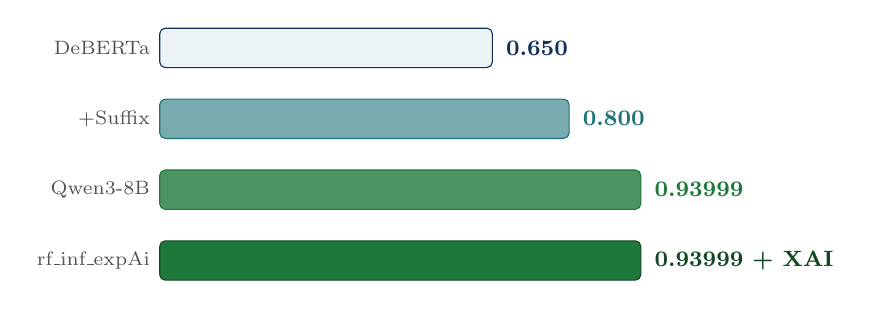
\begin{tikzpicture}
  % Progress bar style
  \draw[fill=RowTintB, draw=TitleBlue, rounded corners=2pt]
    (0, 3.0) rectangle (6.5*0.650, 3.5) node[midway,font=\footnotesize,white] {};
  \node[right, font=\footnotesize\bfseries, color=TitleBlue] at (6.5*0.650+0.05, 3.25) {0.650};
  \node[left, font=\scriptsize, color=SoftGray] at (0, 3.25) {DeBERTa};

  \draw[fill=AccentTeal!60, draw=AccentTeal, rounded corners=2pt]
    (0, 2.1) rectangle (6.5*0.800, 2.6) node[midway,font=\footnotesize,white] {};
  \node[right, font=\footnotesize\bfseries, color=AccentTeal] at (6.5*0.800+0.05, 2.35) {0.800};
  \node[left, font=\scriptsize, color=SoftGray] at (0, 2.35) {+Suffix};

  \draw[fill=GreenOk!80, draw=GreenOk, rounded corners=2pt]
    (0, 1.2) rectangle (6.5*0.940, 1.7) node[midway,font=\footnotesize,white] {};
  \node[right, font=\footnotesize\bfseries, color=GreenOk] at (6.5*0.940+0.05, 1.45) {0.93999};
  \node[left, font=\scriptsize, color=SoftGray] at (0, 1.45) {Qwen3-8B};

  \draw[fill=GreenOk, draw=GreenOk!60!black, rounded corners=2pt]
    (0, 0.3) rectangle (6.5*0.940, 0.8) node[midway,font=\footnotesize,white] {};
  \node[right, font=\footnotesize\bfseries, color=GreenOk!60!black] at (6.5*0.940+0.05, 0.55) {0.93999 + XAI};
  \node[left, font=\scriptsize, color=SoftGray] at (0, 0.55) {rf\_inf\_expAi};
\end{tikzpicture}
\end{center}
\vspace{8pt}
\begin{exampleblock}{Takeaway}
The final system achieves the same classification score as the simple 8B inference, but adds \textbf{full pipeline robustness} and \textbf{natural-language explanations} --- making it both accurate and explainable.
\end{exampleblock}
\end{columns}
\end{frame}

% ============================================================
\section{References}
% ============================================================

% ------ PAPERS 1 --------------------------------------------
\begin{frame}{Research Papers Referenced (1/2)}
\scriptsize
\setlength{\tabcolsep}{3pt}
\renewcommand{\arraystretch}{1.2}
\begin{tabular}{p{0.6cm}p{3.2cm}p{7.0cm}}
\toprule
\textbf{ID} & \textbf{Authors (Year)} & \textbf{Contribution to This Project}\\
\midrule
\rowcolor{RowTintA}
{[M1]} & Vaswani et al.\ (2017) & Transformer architecture --- base of Qwen3-8B \& Qwen2.5-7B\\
{[M2]} & Devlin et al.\ (2019) & BERT fine-tuning paradigm --- DeBERTa \& Qwen classification head design\\
\rowcolor{RowTintA}
{[M3]} & Bai et al.\ (2023) & Qwen technical report --- Stage 1 classifier model\\
{[M4]} & Yang et al.\ (2024) & Qwen2 report --- LLM scorer \& XAI explainer model\\
\rowcolor{RowTintA}
{[M5]} & Ouyang et al.\ (2022) & InstructGPT/RLHF --- instruction-following for JSON KB scoring\\
{[P1]} & Hu et al.\ (2022) & LoRA --- adapter fine-tuning on frozen Qwen3-8B\\
\rowcolor{RowTintA}
{[P2]} & Dettmers et al.\ (2023) & QLoRA --- 4-bit NF4 training; entire 8B model in 16 GB VRAM\\
{[P3]} & Mangrulkar et al.\ (2022) & PEFT library --- \texttt{PeftModel.from\_pretrained()} for adapter loading\\
\rowcolor{RowTintA}
{[P4]} & Dettmers et al.\ (2022) & LLM.int8() / bitsandbytes --- quantization backend\\
{[R1]} & Wu et al.\ (2020) & AWP --- +1.0--2.0\% MAP gain in training\\
\rowcolor{RowTintA}
{[R2]} & Liang et al.\ (2021) & R-Drop --- +0.5--1.5\% MAP gain in training\\
{[R3]} & Tarvainen \& Valpola (2017) & EMA (Mean Teacher) --- +0.3--0.8\% MAP gain\\
\rowcolor{RowTintA}
{[R4][R5]} & M\"uller 2019, Szegedy 2016 & Label smoothing --- prevents overconfident 2587-class head\\
{[R6]} & Loshchilov \& Hutter (2019) & AdamW --- optimizer with decoupled weight decay\\
\rowcolor{RowTintA}
{[R7]} & Howard \& Ruder (2018) & ULMFiT layerwise LR decay (0.95$\times$ per layer)\\
{[R8]} & Pascanu et al.\ (2013) & Gradient clipping (max\_norm = 1.0)\\
\bottomrule
\end{tabular}
\end{frame}

% ------ PAPERS 2 --------------------------------------------
\begin{frame}{Research Papers Referenced (2/2)}
\scriptsize
\setlength{\tabcolsep}{3pt}
\renewcommand{\arraystretch}{1.2}
\begin{tabular}{p{0.6cm}p{3.2cm}p{7.0cm}}
\toprule
\textbf{ID} & \textbf{Authors (Year)} & \textbf{Contribution to This Project}\\
\midrule
\rowcolor{RowTintA}
{[G1]} & Lewis et al.\ (2020) & RAG --- KB retrieval stage; cited in \texttt{retrieve\_context.py}\\
{[G2]} & Edge et al.\ (2024) & GraphRAG --- bounded-subgraph retrieval from ontology graph\\
\rowcolor{RowTintA}
{[G3]} & Jiang et al.\ (2023) & StructGPT --- structured KB entry $\rightarrow$ natural-language LLM context\\
{[G4]} & Luo et al.\ (2024) & RoG (Reasoning on Graphs) --- LLM reasons along graph paths\\
\rowcolor{RowTintA}
{[CF1]} & Wu et al.\ (2021) & Polyjuice --- counterfactual rewriting for causal analysis\\
{[CF3]} & Wu et al.\ (2024) & Counterfactual LLM evaluation --- \texttt{causal\_delta} scoring logic\\
\rowcolor{RowTintA}
{[K1]} & Hogan et al.\ (2021) & Knowledge Graphs survey --- node/edge design for misconception graph\\
{[K2]} & Hagberg et al.\ (2008) & NetworkX --- graph construction, GEXF export, ego-graph queries\\
\rowcolor{RowTintA}
{[K3]} & Rittle-Johnson et al.\ (2025) & Neuro-symbolic educational KGs --- edge types \& KB schema design\\
{[E1]} & Chen \& Guestrin (2016) & XGBoost --- optional meta-learner reranker (70/30 blend)\\
\rowcolor{RowTintA}
{[E2]} & Breiman (1996) & Ensemble stacking --- 14-feature fusion motivation\\
{[T1]} & Salton \& Buckley (1988) & TF-IDF --- baseline retrieval fallback path\\
\rowcolor{RowTintA}
{[T2]} & Manning et al.\ (2008) & MAP@3 metric definition\\
{[EV1]} & J\"arvelin \& Kek\"al\"ainen (2002) & Graded relevance / AP formula\\
\rowcolor{RowTintA}
{[EV2]} & Pedregosa et al.\ (2011) & Scikit-learn --- StratifiedGroupKFold, TfidfVectorizer, LabelEncoder\\
{[XAI1]} & Ribeiro et al.\ (2016) & LIME --- motivation for Phase 2 natural-language explanations\\
\rowcolor{RowTintA}
{[XAI2]} & Lundberg \& Lee (2017) & SHAP --- motivation for hand-tuned 14-feature importance weights\\
{[ED2][ED3]} & Smith 1994, Stacey 1997 & Math misconception theory --- KB field design\\
\bottomrule
\end{tabular}
\end{frame}

% ============================================================
\section{Conclusion}
% ============================================================

% ------ CONCLUSION ------------------------------------------
\begin{frame}{Conclusion}
\begin{columns}[T]
\column{0.50\textwidth}
\begin{block}{What We Built}
A \textbf{six-stage, reproducible pipeline} for automatic math misconception detection:
\begin{enumerate}
  \item Started with DeBERTa-v3 baseline (MAP@3 = 0.65)
  \item Discovered that \textbf{label representation matters} --- suffix classification gave +0.15
  \item Scaled to Qwen3-8B with \textbf{QLoRA + AWP + R-Drop + EMA} --- gave +0.14
  \item Wrapped the classifier with a \textbf{Knowledge Base, Ontology Graph, GraphRAG, and Counterfactual} pipeline
  \item Added \textbf{Explainable AI} --- Qwen3-8B re-used as a text generator to produce natural-language rationales
\end{enumerate}
\end{block}
\column{0.46\textwidth}
\begin{block}{Key Takeaways}
\begin{itemize}
  \item \textbf{Representation design} (suffix labels) can outperform model-scale changes.
  \item \textbf{Parameter-efficient fine-tuning} (QLoRA) makes billion-parameter models practical on consumer GPU.
  \item \textbf{Stacking diverse signals} (KB, graph, counterfactual, classifier) adds robustness beyond what a single model can achieve.
  \item \textbf{Explainability} is not just a nice-to-have --- for an educational tool, it is essential for teacher trust.
\end{itemize}
\end{block}
\vspace{6pt}
\begin{exampleblock}{Final Score}
\begin{center}
\Large MAP@3 = \textbf{0.93999} \quad + \texttt{explanations.json}
\end{center}
\end{exampleblock}
\end{columns}
\end{frame}

% ------ THANK YOU -------------------------------------------
\section{Thank You}
\begin{frame}{Thank You}
\begin{center}
{\Large Questions?}

\vspace{1.2em}

\begin{block}{Summary of Outputs}
\begin{tabular}{ll}
\textbf{submission.csv} & Top-3 ranked misconceptions per student row\\
\textbf{explanations.json} & Natural-language XAI explanation per prediction\\
\textbf{rf\_results/} & Full 14-feature scored candidates (intermediate artifacts)\\
\textbf{graph.gexf} & Inspectable misconception ontology graph\\
\textbf{misconception\_kb.json} & Knowledge base (trigger patterns, cognitive roots, etc.)\\
\end{tabular}
\end{block}

\vspace{1em}
{\small Appendix slides available on request: ablation study, qualitative XAI examples, notebook dependency chain, full paper list.}
\end{center}
\end{frame}

% ============================================================
% APPENDIX
% ============================================================
\appendix
\section{Appendix}

\begin{frame}{Appendix: Full Notebook Dependency Chain}
\begin{center}
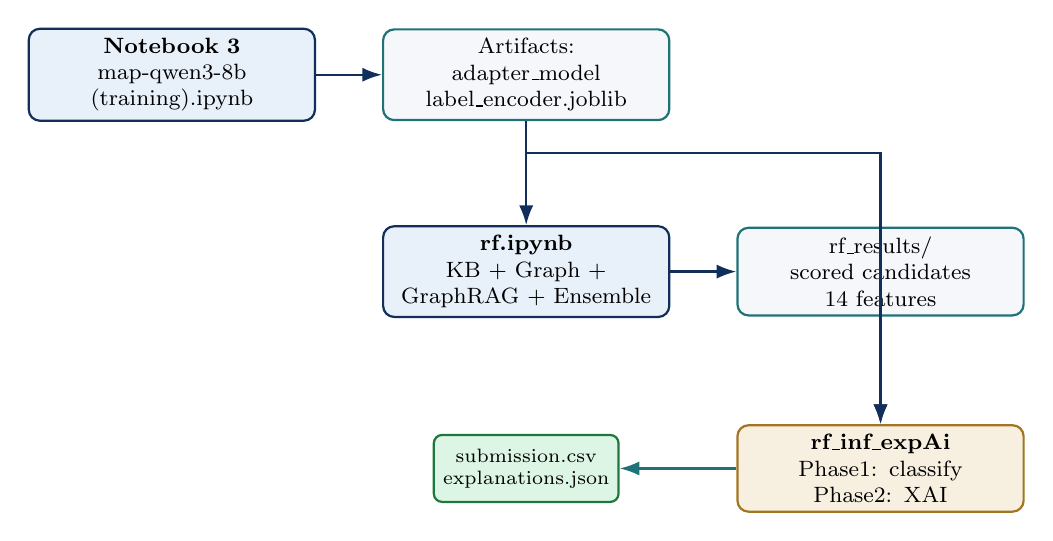
\begin{tikzpicture}
  \node[pipeboxA] (nb3)  at (0, 2.5)  {\textbf{Notebook 3}\\map-qwen3-8b\\(training).ipynb};
  \node[pipeboxB] (art)  at (4.5, 2.5) {Artifacts:\\adapter\_model\\label\_encoder.joblib};
  \node[pipeboxA] (rf)   at (4.5, 0)   {\textbf{rf.ipynb}\\KB + Graph +\\GraphRAG + Ensemble};
  \node[pipeboxB] (res)  at (9.0, 0)   {rf\_results/\\scored candidates\\14 features};
  \node[pipeboxC] (fin)  at (9.0,-2.5) {\textbf{rf\_inf\_expAi}\\Phase1: classify\\Phase2: XAI};
  \node[pipeboxSG](out)  at (4.5,-2.5) {submission.csv\\explanations.json};
  %
  \draw[pipearrow] (nb3) -- (art);
  \draw[pipearrow] (art) -- (rf);
  \draw[pipearrow] (rf)  -- (res);
  \draw[pipearrow] (res) -- (fin);
  \draw[pipearrow] (art.south) -- ++(0,-0.4) -| (fin.north);
  \draw[pipearrowG] (fin) -- (out);
\end{tikzpicture}
\end{center}
\end{frame}

\begin{frame}{Appendix: Ablation --- Each Stage's MAP@3 Contribution}
\small
\begin{center}
\setlength{\tabcolsep}{8pt}
\renewcommand{\arraystretch}{1.3}
\begin{tabular}{lcc}
\toprule
\textbf{Configuration} & \textbf{MAP@3} & \textbf{$\Delta$ vs.\ prev.}\\
\midrule
DeBERTa-v3-Large baseline & 0.650 & ---\\
+ Suffix label representation & 0.800 & +0.150\\
+ Qwen3-8B (QLoRA only, no regularization) & $\approx$0.910 & +0.110\\
+ AWP (awp\_lr=0.1, $\varepsilon$=1e-4) & $\approx$0.926 & +0.016\\
+ R-Drop ($\alpha$=0.5) & $\approx$0.933 & +0.007\\
+ EMA (decay=0.999) & $\approx$0.937 & +0.004\\
+ Label smoothing & 0.93999 & +0.003\\
+ GraphRAG + Counterfactual + Ensemble & 0.93999 & $\approx$0 (robustness)\\
\bottomrule
\end{tabular}
\end{center}
\vspace{8pt}
\begin{block}{Note}
The +0.14 gain from ``DeBERTa+Suffix $\to$ Qwen3-8B+all tricks'' is a combined effect. Individual regularization gains are reported from the training notebook documentation and are approximate (measured on validation folds, not the leaderboard).
\end{block}
\end{frame}

\begin{frame}{Appendix: Why MAP@3 and Not Accuracy?}
\begin{columns}[T]
\column{0.50\textwidth}
\begin{block}{The Competition Rationale}
A teacher reviewing student work does not need the model to be \textit{always perfectly right}. They need the model to \textit{almost always include the correct answer in its top-3 suggestions}.\\[6pt]
MAP@3 rewards:
\begin{itemize}
  \item Being right at rank 1 (score = 1.0) more than rank 2 (score = 0.5) or rank 3 (score = 0.33).
  \item Being \textit{consistent} across all test rows.
\end{itemize}
\end{block}
\column{0.46\textwidth}
\begin{block}{MAP@3 Formula}
For a single test row where the correct misconception is found at rank $r \in \{1, 2, 3\}$:
\[
  \text{AP@3} = \frac{1}{r}
\]
If not found in top-3: AP@3 = 0.

Final score:
\[
  \text{MAP@3} = \frac{1}{N}\sum_{i=1}^{N} \text{AP@3}_i
\]
where $N$ = number of test rows.
\end{block}
\end{columns}
\end{frame}

\end{document}
